\documentclass[8pt,a4paper]{article}

% --- Page Geometry & Margins ---
\usepackage[a4paper, left=7mm, right=7mm, top=7mm, bottom=7mm]{geometry}

% --- Typography ---
\usepackage[utf8]{inputenc}
\usepackage[T1]{fontenc}
\usepackage{helvet}
\renewcommand{\familydefault}{\sfdefault}
\usepackage{microtype}

% --- Graphics & Colors ---
\usepackage{graphicx}
\graphicspath{{Report/figures/}{images/}}
\usepackage{xcolor}
\usepackage{tikz}
\usepackage[most]{tcolorbox}
\usepackage{tabularx}
\usepackage{enumitem}

% --- Spacing & List Compression ---
\setlist{nosep, leftmargin=8pt, itemsep=0.8pt}
\setlength{\parindent}{0pt}
\setlength{\parskip}{0pt}

% --- Hyperlinks ---
\usepackage[hidelinks]{hyperref}

% --- Color Palette ---
\definecolor{navyDark}{HTML}{0A192F}      % Deep Navy
\definecolor{steelBlue}{HTML}{1B4965}     % Primary Blue
\definecolor{accentCyan}{HTML}{0077B6}    % Accent Blue
\definecolor{boxBg}{HTML}{F8FAFC}         % Card Background
\definecolor{boxBorder}{HTML}{CBD5E1}     % Border Gray
\definecolor{badgeBg}{HTML}{E2E8F0}       % Badge Background
\definecolor{badgeText}{HTML}{0F172A}     % Badge Text
\definecolor{textDark}{HTML}{1E293B}      % Body Dark Text

% --- TColorBox Style ---
\tcbset{
    enhanced,
    boxrule=0.5pt,
    arc=2pt,
    left=4pt, right=4pt, top=3pt, bottom=3pt,
    colback=boxBg,
    colframe=boxBorder,
    fonttitle=\bfseries\fontsize{7.5}{8.5}\selectfont,
    coltitle=white,
    attach boxed title to top left={yshift=-1.8mm, xshift=2.5mm},
    boxed title style={
        sharp corners,
        rounded corners=north,
        arc=1.5pt,
        boxrule=0pt,
        colback=steelBlue,
        top=0.8pt, bottom=0.8pt, left=3pt, right=3pt
    }
}

% --- Macros ---
\newcommand{\badge}[1]{%
    \tikz[baseline=(char.base)]{%
        \node[fill=badgeBg, text=badgeText, font=\bfseries\fontsize{5.8}{6.8}\selectfont, inner sep=1.8pt, rounded corners=1.2pt] (char) {#1};%
    }%
}

\newcommand{\kitem}[2]{{\fontsize{6.8}{7.8}\selectfont\textbf{\color{steelBlue}#1:} #2}}
\newcommand{\secsubhead}[1]{{\fontsize{7.2}{8.2}\selectfont\textbf{\color{navyDark}#1}}}

\pagestyle{empty}

\begin{document}

% ==================== HEADER BANNER ====================
\begin{tcolorbox}[
    colback=navyDark,
    colframe=navyDark,
    boxrule=0pt,
    arc=2.5pt,
    top=3pt, bottom=3pt, left=5pt, right=5pt,
    colupper=white
]
    \begin{minipage}[c]{0.72\textwidth}
        {\fontsize{11.5}{13}\bfseries\color{white} STEVE: ROS 2 Autonomous Robot Butler \& Mobile Manipulator} \\[1pt]
        {\fontsize{6.8}{8}\selectfont\color{white!92}
        \textbf{Humanoid Robots Lab (HRL) $\cdot$ University of Bonn} $\;\vert\;$ Supervisor: Rohit Menon $\;\vert\;$ Lab Head: Prof. Dr. Maren Bennewitz} \\[1.5pt]
        {\fontsize{6.3}{7.5}\selectfont\color{white!80}
        \textbf{Core Developers:} Shrikar Nakhye $\cdot$ Pratik Adhikari $\cdot$ Riddhesh More \quad $\vert$ \quad \textbf{Workspace:} \texttt{steve\_ros2\_ws} (ROS 2 Humble)}
    \end{minipage}%
    \hfill
    \begin{minipage}[c]{0.27\textwidth}
        \flushright
        \badge{ROS 2 Humble} \ \badge{Neobotix MMO-700} \ \badge{UR5e 6-DoF} \\[1.5pt]
        \badge{Nav2 + A*} \ \badge{RTAB-Map 3D} \ \badge{SAM3 + DeepSeek}
    \end{minipage}
\end{tcolorbox}

\vspace{-4pt}

% ==================== MAIN 2-COLUMN LAYOUT ====================
\begin{minipage}[t]{0.485\textwidth}

    % --- Box 1: Platform & Hardware ---
    \begin{tcolorbox}[title={Robot Platform \& Hardware Specs}]
        \begin{tabularx}{\linewidth}{@{} l X @{}}
            \kitem{Mobile Base}{Neobotix MMO-700 Omnidirectional (4-wheel omnidrive)} \\
            \kitem{Manipulator}{Universal Robots UR5e 6-DoF Arm + Robotiq 2F-85 Gripper} \\
            \kitem{Perception Head}{Intel RealSense L515 on Dynamixel XL430-W250 Pan-Tilt Unit} \\
            \kitem{Safety LiDAR}{Dual SICK S300 Laser Scanners ($360^\circ$ planar safety coverage)} \\
            \kitem{System Bringup}{\texttt{ROS\_AUTOSTART.sh} in \texttt{screen} daemon; static IP / DHCP} \\
        \end{tabularx}
    \end{tcolorbox}

    \vspace{-4pt}

    % --- Box 2: System Architecture ---
    \begin{tcolorbox}[title={Layered Software Architecture}]
        \centering
        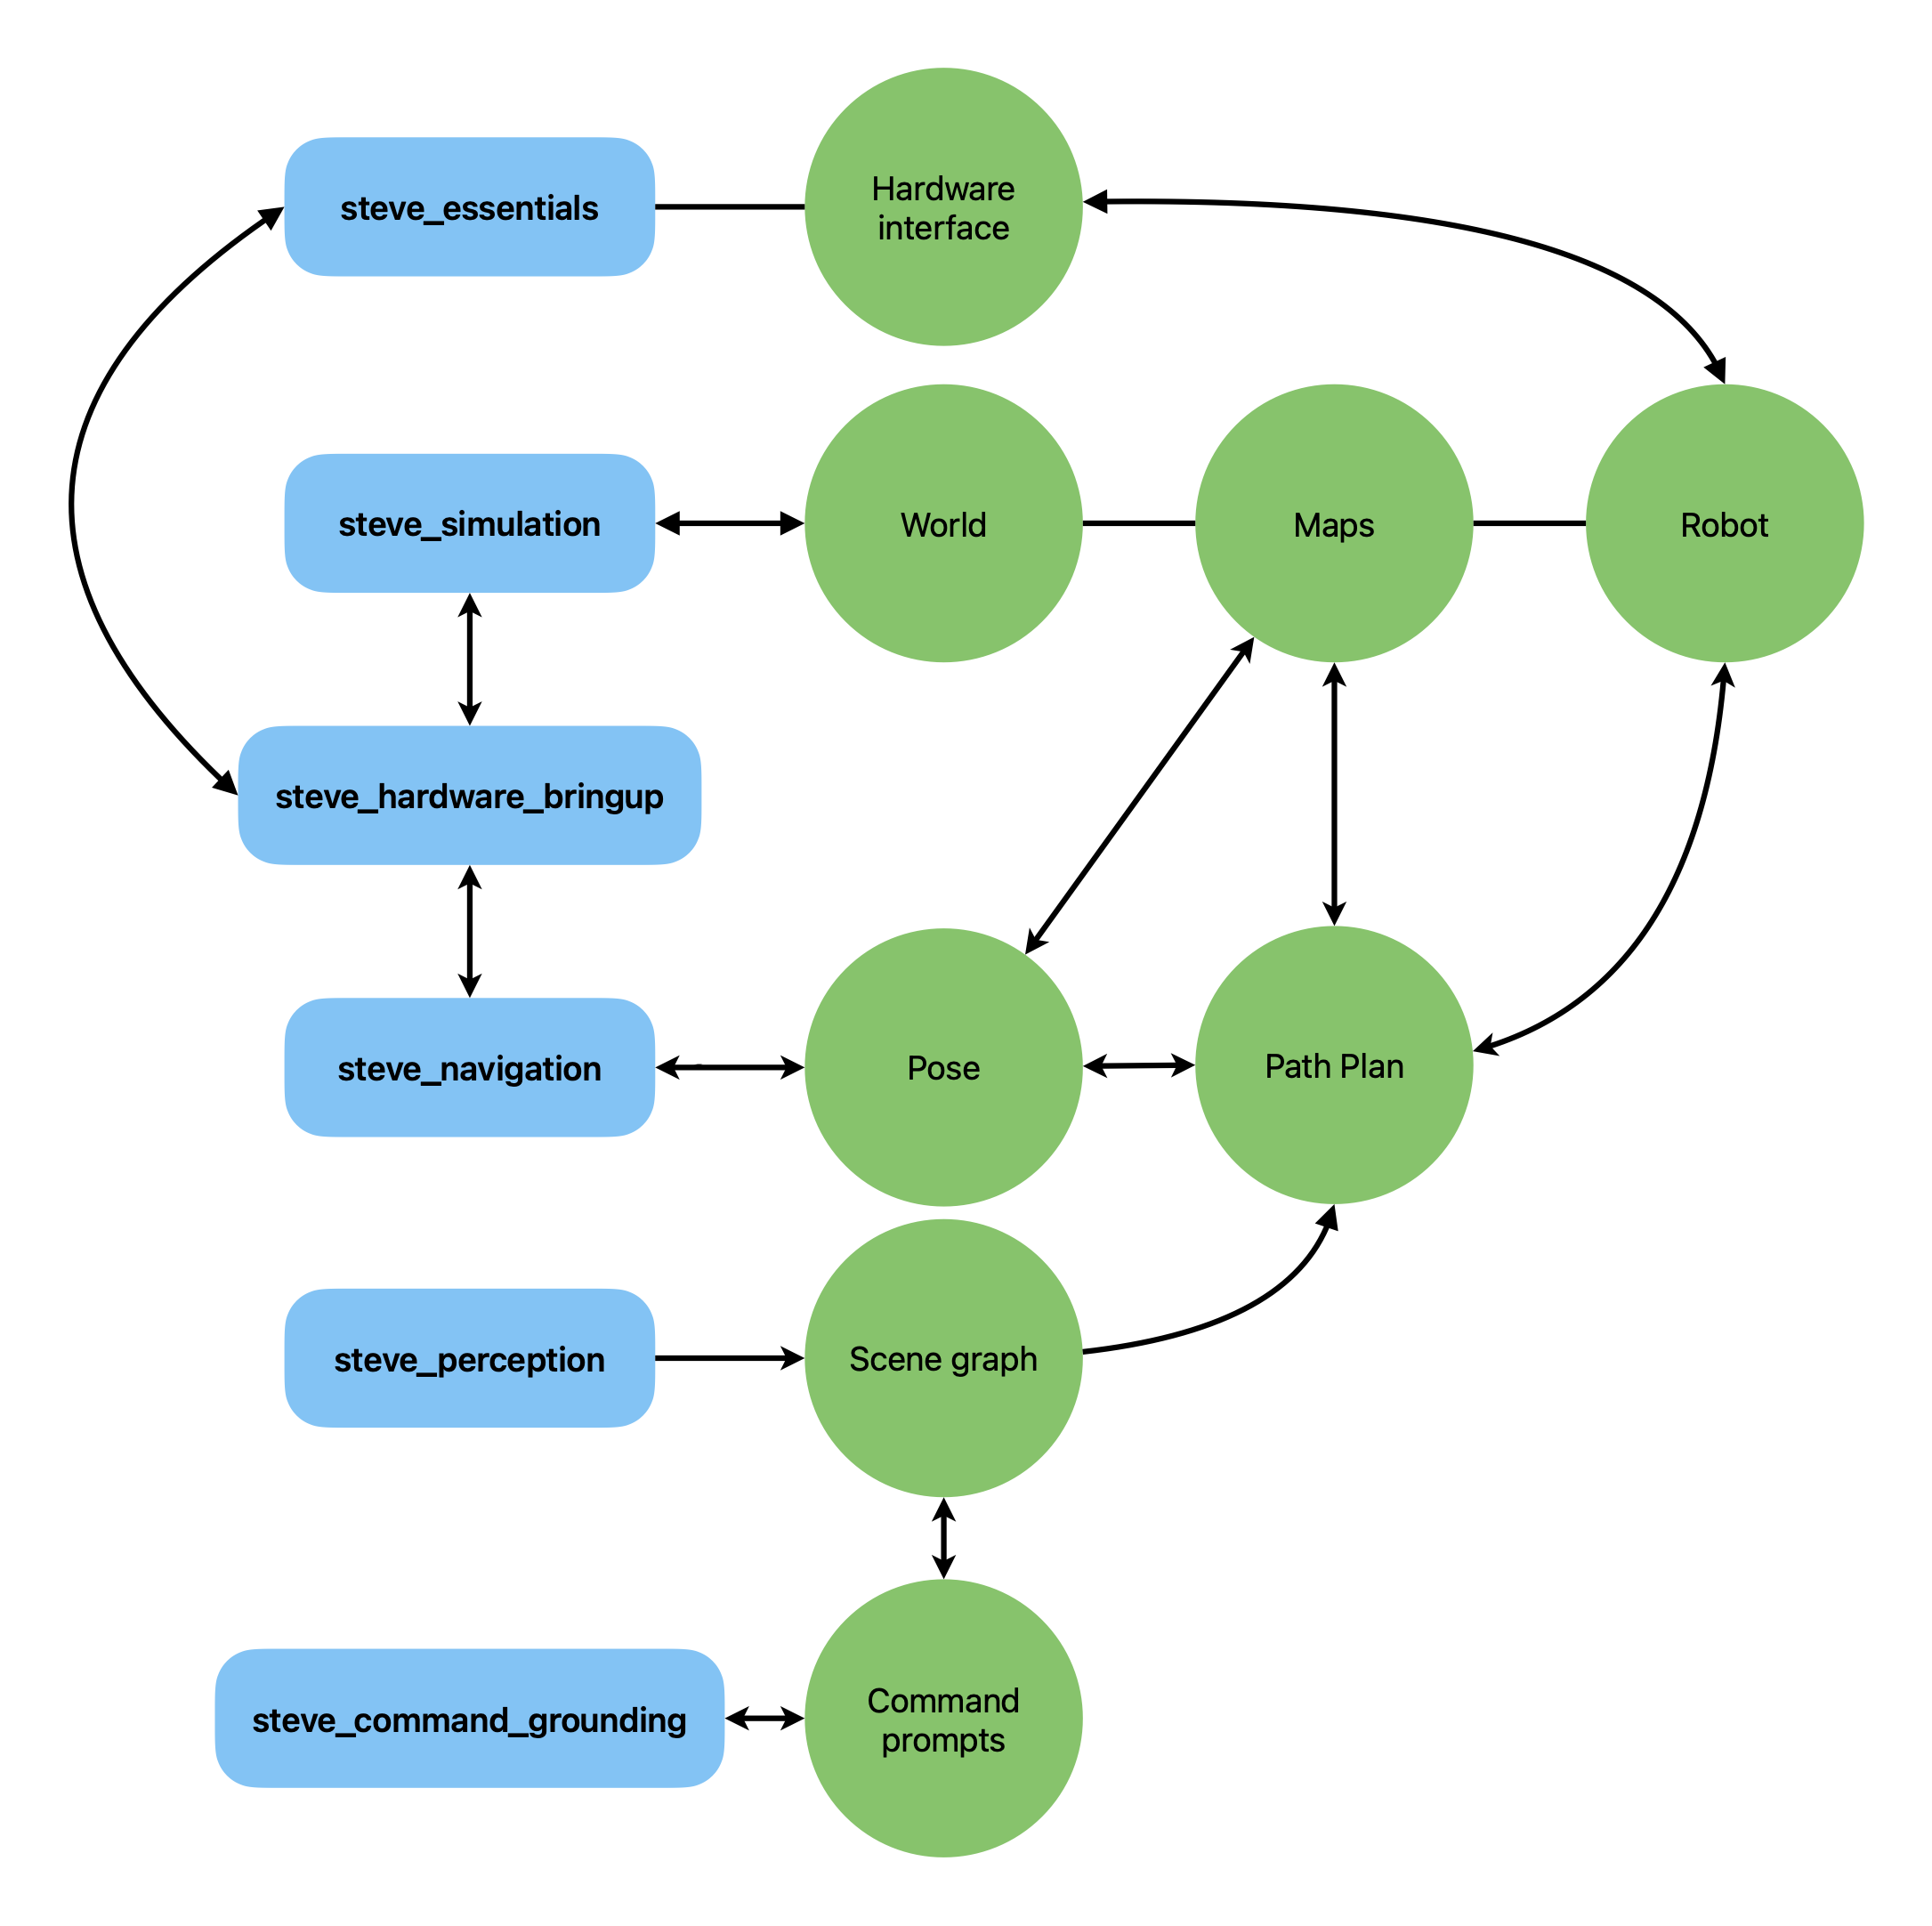
\includegraphics[width=0.96\linewidth, height=3.0cm, keepaspectratio]{Steve_architecture}
        \vspace{1pt}
        \begin{itemize}
            \item \kitem{\texttt{steve\_essentials}}{Hardware drivers (Base, LiDAR, L515), \texttt{neo\_msgs2}, kinematics.}
            \item \kitem{\texttt{steve\_hardware\_bringup}}{Synchronized startup of base, arm, and sensors without race conditions.}
            \item \kitem{\texttt{steve\_simulation}}{High-fidelity Gazebo digital twin with URDF/Xacro parity.}
            \item \kitem{Docker AI Services}{Isolated GPU containers for heavy AI models (Mask3D, SAM3).}
        \end{itemize}
    \end{tcolorbox}

    \vspace{-4pt}

    % --- Box 3: Simulation & RViz Visuals ---
    \begin{tcolorbox}[title={Simulation \& Visualization Environments}]
        \begin{minipage}[c]{0.48\textwidth}
            \centering
            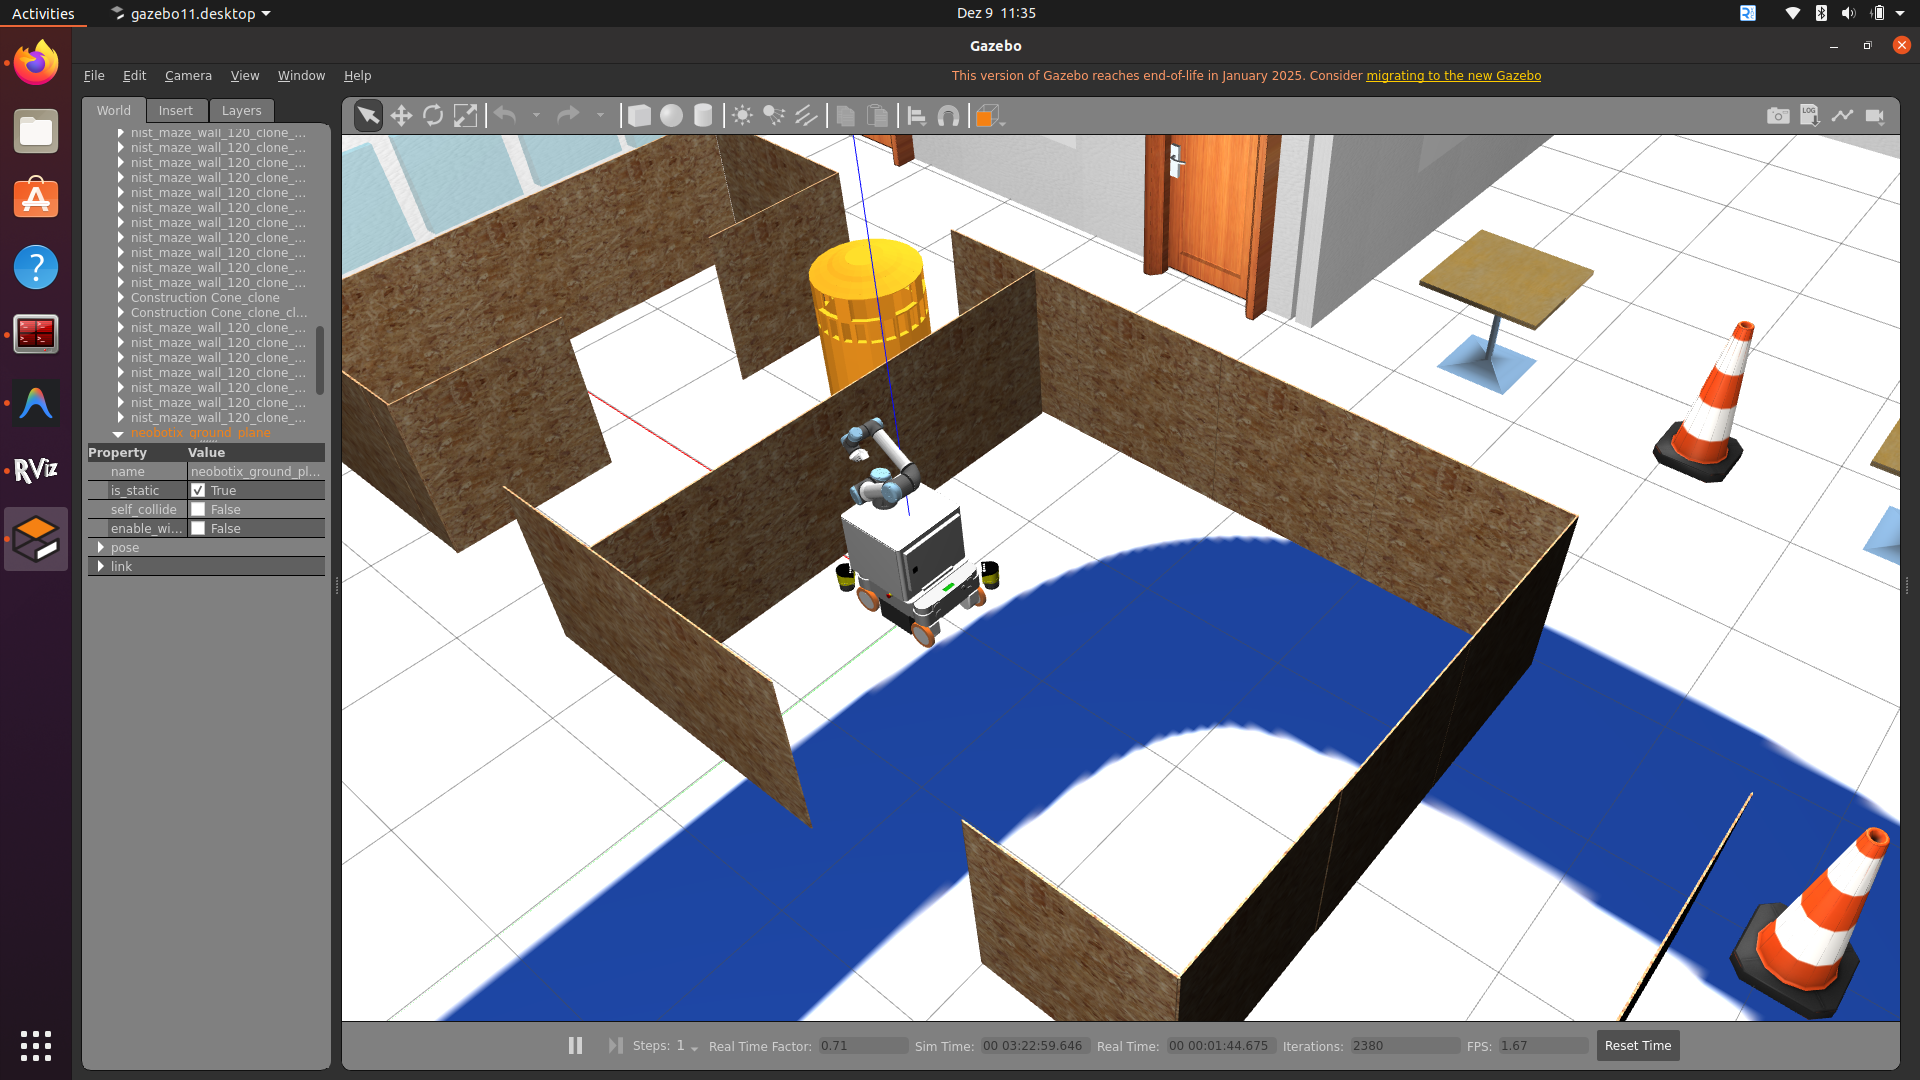
\includegraphics[width=\linewidth, height=1.65cm, keepaspectratio]{gazebo.png} \\[0.5pt]
            {\fontsize{5.8}{6.8}\selectfont\textbf{Gazebo (\texttt{steve\_house})}}
        \end{minipage}%
        \hfill
        \begin{minipage}[c]{0.48\textwidth}
            \centering
            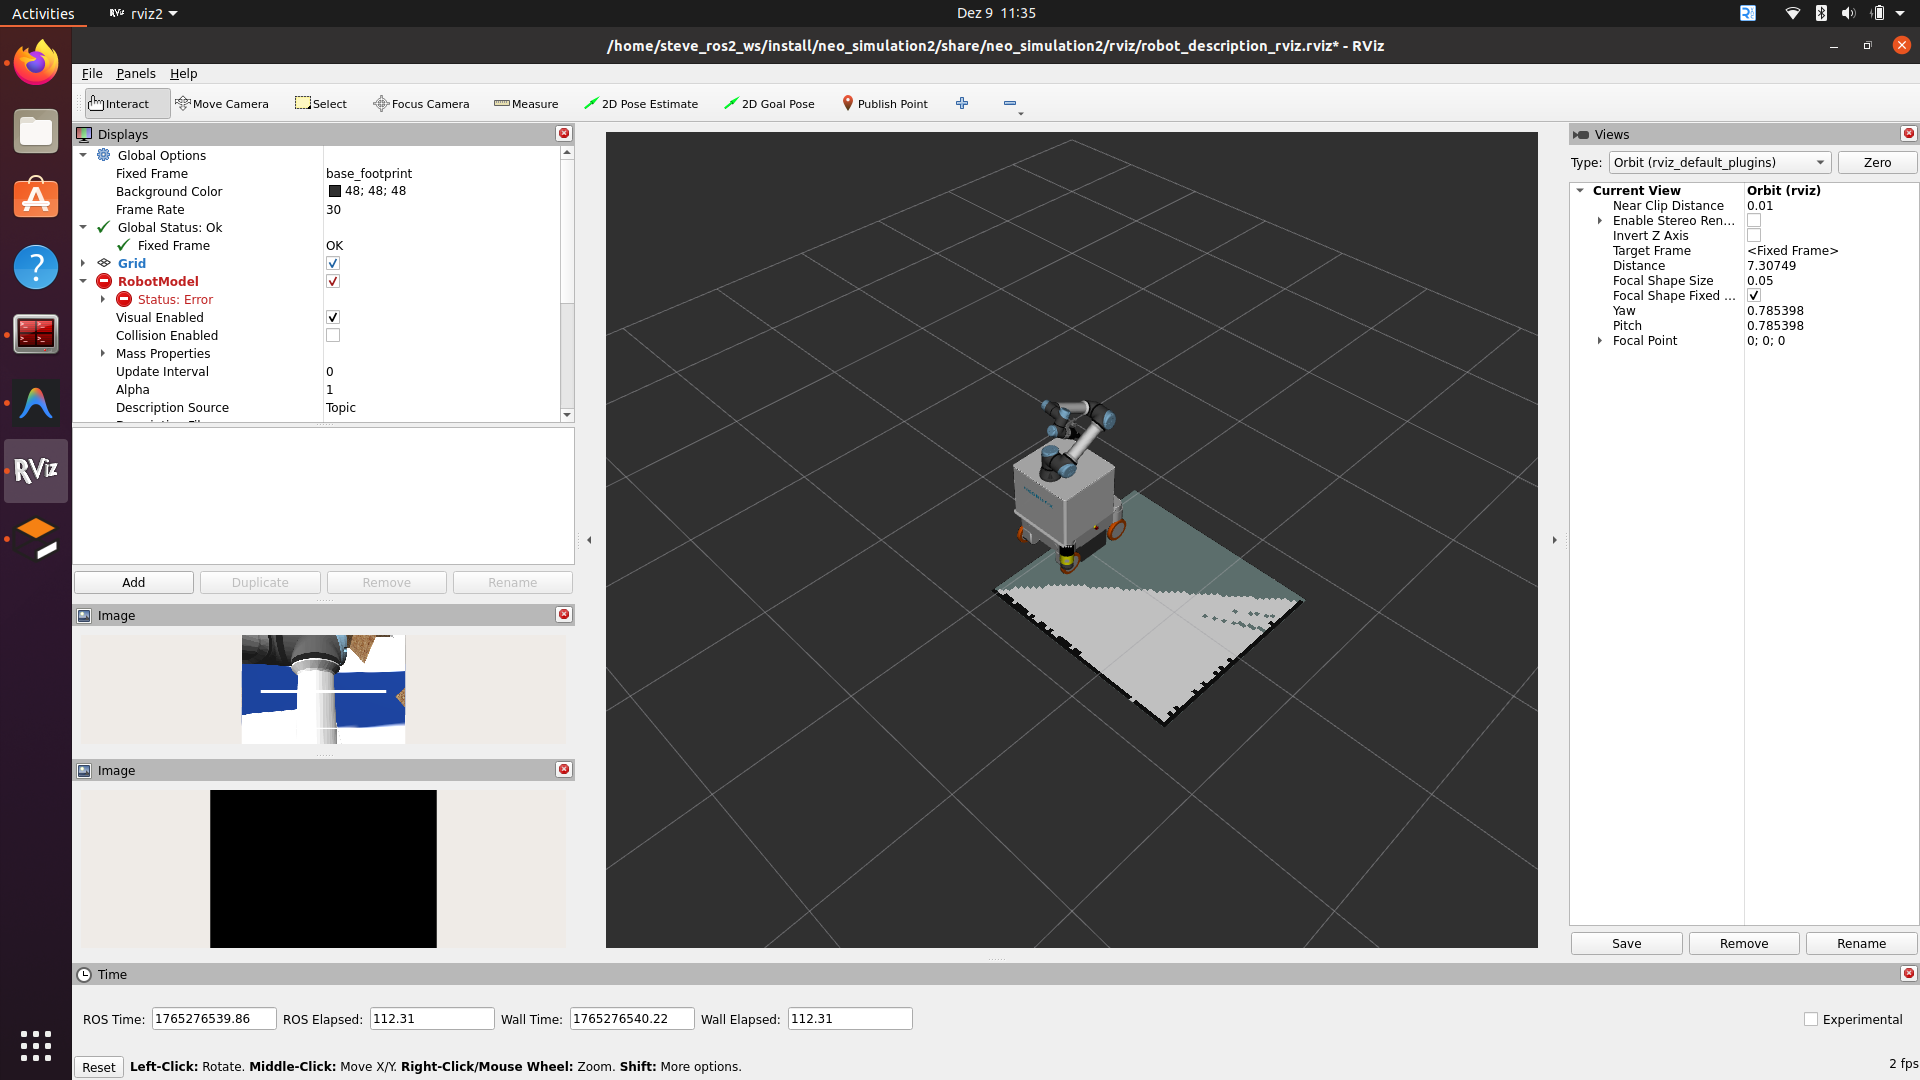
\includegraphics[width=\linewidth, height=1.65cm, keepaspectratio]{rviz.png} \\[0.5pt]
            {\fontsize{5.8}{6.8}\selectfont\textbf{Nav2 + SLAM in RViz2}}
        \end{minipage}
        \vspace{1pt}
        \begin{itemize}
            \item \kitem{Simulation Worlds}{\texttt{steve\_house}, \texttt{small\_house}, and \texttt{neo\_workshop}.}
            \item \kitem{Deployment Profiles}{Config profiles for simulation, hardware, and rosbag replay.}
        \end{itemize}
    \end{tcolorbox}

\end{minipage}%
\hfill
\begin{minipage}[t]{0.495\textwidth}

    % --- Box 4: Navigation, Perception & Reasoning Pipeline ---
    \begin{tcolorbox}[title={Autonomy, Perception \& Reasoning Stack}]
        \secsubhead{1. Autonomous Navigation \& Localization (Nav2)}
        \begin{itemize}
            \item \kitem{A* Global Planning}{Replaced default Dijkstra with A* heuristic for rapid, optimal path search in narrow domestic and workshop passages.}
            \item \kitem{AMCL Particle Filter Tuning}{Increased particle thresholds and update rates to eliminate robot kidnapping in symmetric, feature-sparse environments.}
            \item \kitem{Sim-to-Real Transfer}{Unified TF tree and topics for seamless sim-to-real code reuse.}
        \end{itemize}
        \vspace{2pt}

        \secsubhead{2. 3D Semantic Mapping \& Scene Graphs (RTAB-Map)}
        \begin{itemize}
            \item \kitem{Bandwidth Optimization}{Compressed \texttt{RGBDImage} transport (JPEG+Uint16) achieving $\approx$90\% serialization reduction (0.8\,MB vs 8\,MB/frame).}
            \item \kitem{RANSAC + DBSCAN}{Horizontal plane detection ($\mathbf{n}\cdot[0,0,1]\ge0.95$) with 2D plane-tangent clustering to cleanly isolate floors from obstacles.}
            \item \kitem{Scene Graph Generation}{PCA-based Oriented Bounding Boxes (OBB), support planes ($\mathbf{n}_z>0.9$), and containment relations for domestic objects.}
        \end{itemize}
        \vspace{2pt}

        \secsubhead{3. Open-Vocabulary Command Grounding (LLM + SAM3)}
        \begin{itemize}
            \item \kitem{DeepSeek-R1 Commonsense LLM}{Infers likely target locations (e.g., ``water bottle $\to$ kitchen table'') when objects are unindexed in scene graph.}
            \item \kitem{SAM3 Zero-Shot Vision}{Containerized prompt-based visual segmentation and 3D raycasting to project camera detections into global map coordinates.}
            \item \kitem{Collision-Aware Standoff}{FOV-based standoff position optimization with Open3D point-cloud collision checks for unobstructed surface inspection.}
        \end{itemize}
    \end{tcolorbox}

    \vspace{-4pt}

    % --- Box 5: Key Engineering Achievements ---
    \begin{tcolorbox}[title={Key Engineering Achievements \& Benchmarks}]
        \begin{itemize}
            \item \kitem{Network Bandwidth}{90\% DDS serialization reduction via compressed RGBD feeds.}
            \item \kitem{TF Sanitization Relay}{Fixed historical bag jumps/orphans, raising replay from 40\% to \textbf{95\%}.}
            \item \kitem{GPU Acceleration}{Docker GPU passthrough slashed 3D segmentation from \textbf{40m} to \textbf{2m}.}
            \item \kitem{PTU SyncWrite Driver}{Simultaneous Dynamixel packet writes eliminate inter-motor jitter.}
            \item \kitem{Hands-Off Operation}{Full autostart daemon boots all drivers safely on physical hardware.}
        \end{itemize}
    \end{tcolorbox}

\end{minipage}

\vspace{-4pt}

% ==================== TEAM & CONTRIBUTIONS BREAKDOWN ====================
\begin{tcolorbox}[title={Team Contributions \& Work Package Breakdown}, colback=white]
    \begin{tabularx}{\textwidth}{@{} X X X @{}}
        \textbf{\color{steelBlue}\fontsize{7.2}{8.2}\selectfont Shrikar Nakhye} & 
        \textbf{\color{steelBlue}\fontsize{7.2}{8.2}\selectfont Pratik Adhikari} & 
        \textbf{\color{steelBlue}\fontsize{7.2}{8.2}\selectfont Riddhesh More} \\
        {\fontsize{6.3}{7.4}\selectfont $\bullet$ Core architecture \& modular migration} & 
        {\fontsize{6.3}{7.4}\selectfont $\bullet$ RTAB-Map 3D RGB-D SLAM pipeline} & 
        {\fontsize{6.3}{7.4}\selectfont $\bullet$ DeepSeek-R1 + SAM3 grounding pipeline} \\
        {\fontsize{6.3}{7.4}\selectfont $\bullet$ Centralized bringup \& auto-start daemon} & 
        {\fontsize{6.3}{7.4}\selectfont $\bullet$ RANSAC + DBSCAN plane segmentation} & 
        {\fontsize{6.3}{7.4}\selectfont $\bullet$ Dynamixel XL430 SyncWrite controller} \\
        {\fontsize{6.3}{7.4}\selectfont $\bullet$ Nav2 A* global planner \& AMCL tuning} & 
        {\fontsize{6.3}{7.4}\selectfont $\bullet$ Scene graph generation \& spatial relations} & 
        {\fontsize{6.3}{7.4}\selectfont $\bullet$ Collision-aware standoff visual planner} \\
        {\fontsize{6.3}{7.4}\selectfont $\bullet$ Hardware repair, network \& Git dev workflow} & 
        {\fontsize{6.3}{7.4}\selectfont $\bullet$ TF sanitization relay (95\% replay)} & 
        {\fontsize{6.3}{7.4}\selectfont $\bullet$ Nav2 Action Wrapper \& Gazebo worlds} \\
    \end{tabularx}
\end{tcolorbox}

\end{document}
